\documentclass{beamer}

\usepackage{etex}
\usepackage{myprogram}
\normalbaroutside

\usepackage{tikz}
\usetikzlibrary{matrix}
\usetikzlibrary{calc}
\usetikzlibrary{positioning}
\usepackage{tikz-qtree}

\title{Content Planning for CCG}
\subtitle{A Graph Transformation Toolkit}
\author{Bernd Kiefer\\\texttt{Bernd.Kiefer@dfki.de}}
\institute{Deutsches Forschungszentrum f\"ur k\"unstliche Intelligenz}
\date{November 8, 2010}

\begin{document}
\definecolor[named]{dblue}{rgb}{.1 .1 .62}    % a darker blue
\definecolor[named]{dgreen}{rgb}{0 0.7 0}     % a darker green
\definecolor[named]{dred}{rgb}{0.7 0 0}       % a darker red
\newcommand{\dblue}[1]{\color{dblue}#1}
\newcommand{\dgreen}[1]{\color{dgreen}#1}
\newcommand{\dred}[1]{\color{dred}#1}
\let\origem=\emph
\renewcommand{\emph}[1]{\origem{\dblue #1}}

\pgfdeclareimage[height=0.5cm]{dfkilogo}{dfkiltlight}
\logo{\pgfuseimage{dfkilogo}}

\frame{\titlepage}
\frame{\frametitle{Overview}\tableofcontents}

\section{General Idea}

\begin{frame}[fragile]{Logical Forms as Graphs}

\begin{flushleft}\small
A CCG logical form can be interpreted as an acyclic graph:
\begin{verbatim}
@d1:dvp(<Content>(c1:ascription ^
                  <Cop-Scope>(cs1:type ^ <Questioned>true))
        <Wh-Restr>(:specifier ^ what ^ <Scope> (cs1:type)))
\end{verbatim}
\end{flushleft}

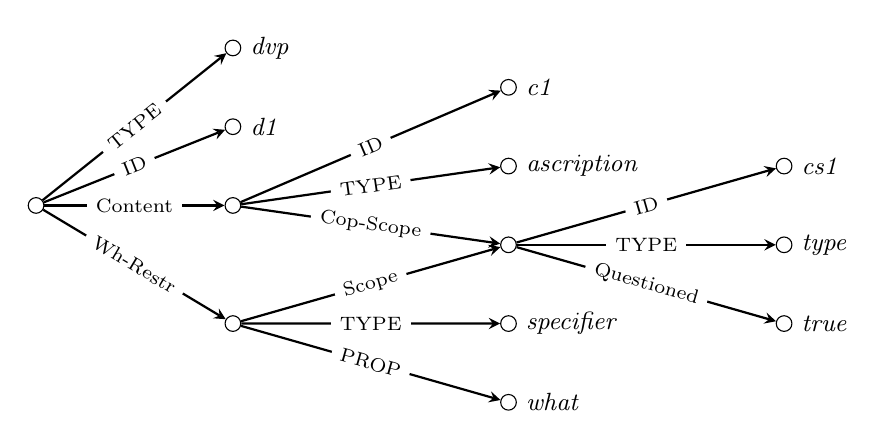
\begin{tikzpicture}[node distance=2cm, font=\scriptsize,
  v/.style={circle, draw, inner sep=2pt},
  edge/.style={draw,thick,-stealth},
  val/.style={anchor=west, xshift=1mm, font=\it\small},
]
%layer zero
\node[v] (root) {};
%layer one
\node[v] (r-cont) [right of=root,  node distance=2.5cm] {};
\node[v] (r-id)   [above of=r-cont, node distance=1cm] {};
\node[val] at (r-id) {d1};
\node[v] (r-type) [above of=r-id, node distance=1cm] {};
\node[val] at (r-type) {dvp};
\node[v] (r-wh) [below of=r-cont, node distance=1.5cm] {};
%layer two
\node[v] (c-scope) [right of=r-cont,node distance=3.5cm,yshift=-.5cm] {};
\node[v] (c-type) [above of=c-scope, node distance=1cm] {};
\node[val] at (c-type) {ascription};
\node[v] (c-id) [above of=c-type, node distance=1cm] {};
\node[val] at (c-id) {c1};
\node[v] (wh-type) [below of=c-scope, node distance=1cm] {};
\node[val] at (wh-type) {specifier};
\node[v] (wh-prop) [below of=wh-type, node distance=1cm] {};
\node[val] at (wh-prop) {what};
%layer three
\node[v] (cs-id)   [right of=c-type,node distance=3.5cm] {};
\node[val] at (cs-id) {cs1};
\node[v] (cs-type) [below of=cs-id, node distance=1cm]  {};
\node[val] at (cs-type) {type};
\node[v] (cs-quest)[below of=cs-type, node distance=1cm] {};
\node[val] at (cs-quest) {true};

\foreach \fr / \tonode / \name in { root/r-id/ID, root/r-type/TYPE,
  root/r-cont/Content, root/r-wh/Wh-Restr, r-cont/c-id/ID, r-cont/c-type/TYPE,
  r-cont/c-scope/Cop-Scope, r-wh/wh-type/TYPE,
  r-wh/wh-prop/PROP, r-wh/c-scope/Scope, c-scope/cs-id/ID,
  c-scope/cs-type/TYPE, c-scope/cs-quest/Questioned }
\draw[edge] (\fr) to node[fill=white, sloped] {\name} (\tonode);
\end{tikzpicture}
\end{frame}

%%%%%%%%%%%%%%%%%%%%%%%%%%%%%%%%%%%%%%%%%%%%%%%%%%%%%%%%%%%%%%%%%%%%%%%%%%%%%%%

\begin{frame}{Content Planning as Graph Transformation}
  \begin{block}{The Content Planner as a Rule System}
    The Planner consists of
    \begin{itemize}
    \item A set of transformation rules that specify the local modifications
    \item A processing engine that applies the rules to all sub-parts of the
      logical form with a specific strategy
    \end{itemize}

  \end{block}
  \begin{block}{Transformation rules: Antecedent and Consequent}
    \begin{itemize}
    \item \textit{Match Part} specify what shape some substructure of the graph
      must exhibit to make it applicable to a rule
    \item \textit{Action Part} specify the modifications to parts of the
      substructure
    \end{itemize}
  \end{block}
\end{frame}

%%%%%%%%%%%%%%%%%%%%%%%%%%%%%%%%%%%%%%%%%%%%%%%%%%%%%%%%%%%%%%%%%%%%%%%%%%%%%%%

\begin{frame}{Step 1: Match Patterns}

\begin{flushleft}\small
Specify patterns where certain actions should be applied\\[2ex]
\only<1>{{\color{dred}\texttt{<TYPE>}} \ \ (activate all nodes that have an
  outgoing TYPE edge)}
\only<2>{{\color{dred}\texttt{<TYPE> ascription}} (alternatively:
 \texttt{:ascription})}
\end{flushleft}

\begin{tikzpicture}[node distance=2cm, font=\scriptsize,
  v/.style={circle, draw, inner sep=2pt},
  edge/.style={draw,thick,-stealth},
  val/.style={anchor=west, xshift=1mm, font=\it\small},
]
%layer zero
\node[v] (root) {};
%layer one
\node[v] (r-cont) [right of=root,  node distance=2.5cm] {};
\node[v] (r-id)   [above of=r-cont, node distance=1cm] {};
\node[val] at (r-id) {d1};
\node[v] (r-type) [above of=r-id, node distance=1cm] {};
\node[val] at (r-type) {dvp};
\node[v] (r-wh) [below of=r-cont, node distance=1.5cm] {};
%layer two
\node[v] (c-scope) [right of=r-cont,node distance=3.5cm,yshift=-.5cm] {};
\node[v] (c-type) [above of=c-scope, node distance=1cm] {};
\node[val] at (c-type) {ascription};
\node[v] (c-id) [above of=c-type, node distance=1cm] {};
\node[val] at (c-id) {c1};
\node[v] (wh-type) [below of=c-scope, node distance=1cm] {};
\node[val] at (wh-type) {specifier};
\node[v] (wh-prop) [below of=wh-type, node distance=1cm] {};
\node[val] at (wh-prop) {what};
%layer three
\node[v] (cs-id)   [right of=c-type,node distance=3.5cm] {};
\node[val] at (cs-id) {cs1};
\node[v] (cs-type) [below of=cs-id, node distance=1cm]  {};
\node[val] at (cs-type) {type};
\node[v] (cs-quest)[below of=cs-type, node distance=1cm] {};
\node[val] at (cs-quest) {true};

\foreach \fr / \tonode / \name in { root/r-id/ID, root/r-type/TYPE,
  root/r-cont/Content, root/r-wh/Wh-Restr, r-cont/c-id/ID, r-cont/c-type/TYPE,
  r-cont/c-scope/Cop-Scope, r-wh/wh-type/TYPE,
  r-wh/wh-prop/PROP, r-wh/c-scope/Scope, c-scope/cs-id/ID,
  c-scope/cs-type/TYPE, c-scope/cs-quest/Questioned }
\draw[edge] (\fr) to node[fill=white, sloped] {\name} (\tonode);

\only<1>{
\begin{scope}[color=dred]
\foreach \fr / \tonode / \name in { root/r-type/TYPE,
 r-cont/c-type/TYPE,
 r-wh/wh-type/TYPE,
  c-scope/cs-type/TYPE }
\draw[edge] (\fr) to node[fill=white, sloped] {\name} (\tonode);
\end{scope}
\begin{scope}[color=dgreen, v/.style={circle, draw, fill=dgreen, inner sep=2pt}]
\node[v] at (root) {};
\node[v] at (r-cont) {};
\node[v] at (r-wh) {};
\node[v] at (c-scope) {};
\end{scope}
}

\only<2>{
\begin{scope}[color=dred]
\foreach \fr / \tonode / \name in { r-cont/c-type/TYPE }
\draw[edge] (\fr) to node[fill=white, sloped] {\name} (\tonode);
\node[v] at (c-type) {};
\node[val] at (c-type) {ascription};
\end{scope}
\begin{scope}[color=dgreen, v/.style={circle, draw, fill=dgreen, inner sep=2pt}]
\node[v] at (r-cont) {};
\end{scope}
}
\end{tikzpicture}
\end{frame}

%%%%%%%%%%%%%%%%%%%%%%%%%%%%%%%%%%%%%%%%%%%%%%%%%%%%%%%%%%%%%%%%%%%%%%%%%%%%%%%

\begin{frame}{Step 2: Actions}

\begin{flushleft}\small
How should the active node be modified\\[2ex]
{\color{dred}\texttt{\# \^\  :newtype}} overwrites the type (shorthand for
\texttt{\# \^\ <TYPE>newtype})
\end{flushleft}

\begin{tikzpicture}[node distance=2cm, font=\scriptsize,
  v/.style={circle, draw, inner sep=2pt},
  edge/.style={draw,thick,-stealth},
  val/.style={anchor=west, xshift=1mm, font=\it\small},
]
%layer zero
\node[v] (root) {};
%layer one
\node[v] (r-cont) [right of=root,  node distance=2.5cm] {};
\node[v] (r-id)   [above of=r-cont, node distance=1cm] {};
\node[val] at (r-id) {d1};
\node[v] (r-type) [above of=r-id, node distance=1cm] {};
\node[val] at (r-type) {dvp};
\node[v] (r-wh) [below of=r-cont, node distance=1.5cm] {};
%layer two
\node[v] (c-scope) [right of=r-cont,node distance=3.5cm,yshift=-.5cm] {};
\node[v] (c-type) [above of=c-scope, node distance=1cm] {};
\node[val] at (c-type) {\only<1>{\color{dred} ascription}};
\node[v] (c-id) [above of=c-type, node distance=1cm] {};
\node[val] at (c-id) {c1};
\node[v] (wh-type) [below of=c-scope, node distance=1cm] {};
\node[val] at (wh-type) {specifier};
\node[v] (wh-prop) [below of=wh-type, node distance=1cm] {};
\node[val] at (wh-prop) {what};
%layer three
\node[v] (cs-id)   [right of=c-type,node distance=3.5cm] {};
\node[val] at (cs-id) {cs1};
\node[v] (cs-type) [below of=cs-id, node distance=1cm]  {};
\node[val] at (cs-type) {type};
\node[v] (cs-quest)[below of=cs-type, node distance=1cm] {};
\node[val] at (cs-quest) {true};

\foreach \fr / \tonode / \name in { root/r-id/ID, root/r-type/TYPE,
  root/r-cont/Content, root/r-wh/Wh-Restr, r-cont/c-id/ID, r-cont/c-type/TYPE,
  r-cont/c-scope/Cop-Scope, r-wh/wh-type/TYPE,
  r-wh/wh-prop/PROP, r-wh/c-scope/Scope, c-scope/cs-id/ID,
  c-scope/cs-type/TYPE, c-scope/cs-quest/Questioned }
\draw[edge] (\fr) to node[fill=white, sloped] {\name} (\tonode);


\begin{scope}[color=dred]
\foreach \fr / \tonode / \name in { r-cont/c-type/TYPE }
\draw[edge] (\fr) to node[fill=white, sloped] {\name} (\tonode);
\node[v] at (c-type) {};
\end{scope}
\begin{scope}[color=dgreen, v/.style={circle, draw, fill=dgreen, inner sep=2pt}]
\node[v] at (r-cont) {};
\node[val] at (c-type) {\only<2->{newtype}};
\end{scope}
\end{tikzpicture}
\end{frame}

%%%%%%%%%%%%%%%%%%%%%%%%%%%%%%%%%%%%%%%%%%%%%%%%%%%%%%%%%%%%%%%%%%%%%%%%%%%%%%%

\begin{frame}{Step 2: Actions}

\begin{flushleft}\small
{\color{dred}\texttt{\# = <Feat> val}} replaces active node with a new node
having only a type attribute
\end{flushleft}

\begin{tikzpicture}[node distance=2cm, font=\scriptsize,
  v/.style={circle, draw, inner sep=2pt},
  edge/.style={draw,thick,-stealth},
  val/.style={anchor=west, xshift=1mm, font=\it\small},
]
%layer zero
\node[v] (root) {};
%layer one
\node[v] (r-cont) [right of=root,  node distance=2.5cm] {};
\node[v] (r-id)   [above of=r-cont, node distance=1cm] {};
\node[val] at (r-id) {d1};
\node[v] (r-type) [above of=r-id, node distance=1cm] {};
\node[val] at (r-type) {dvp};
\node[v] (r-wh) [below of=r-cont, node distance=1.5cm] {};
%layer two
\node[v] (c-scope) [right of=r-cont,node distance=3.5cm,yshift=-.5cm] {};
\node[v] (c-type) [above of=c-scope, node distance=1cm] {};
%\node[v] (c-id) [above of=c-type, node distance=1cm] {};
%\node[val] at (c-id) {c1};
\node[v] (wh-type) [below of=c-scope, node distance=1cm] {};
\node[val] at (wh-type) {specifier};
\node[v] (wh-prop) [below of=wh-type, node distance=1cm] {};
\node[val] at (wh-prop) {what};
%layer three
\node[v] (cs-id)   [right of=c-type,node distance=3.5cm] {};
\node[val] at (cs-id) {cs1};
\node[v] (cs-type) [below of=cs-id, node distance=1cm]  {};
\node[val] at (cs-type) {type};
\node[v] (cs-quest)[below of=cs-type, node distance=1cm] {};
\node[val] at (cs-quest) {true};

\foreach \fr / \tonode / \name in { root/r-id/ID, root/r-type/TYPE,
  root/r-cont/Content, root/r-wh/Wh-Restr,
  r-wh/wh-type/TYPE,
  r-wh/wh-prop/PROP, r-wh/c-scope/Scope, c-scope/cs-id/ID,
  c-scope/cs-type/TYPE, c-scope/cs-quest/Questioned }
\draw[edge] (\fr) to node[fill=white, sloped] {\name} (\tonode);

\begin{scope}[color=dgreen, v/.style={circle, draw, fill=dgreen, inner sep=2pt}]
\foreach \fr / \tonode / \name in { r-cont/c-type/Feat }
\draw[edge] (\fr) to node[fill=white, sloped] {\name} (\tonode);
\node[v] at (r-cont) {};
\node[v] at (c-type) {};
\node[val] at (c-type) {val};
\end{scope}

\end{tikzpicture}
\end{frame}

%%%%%%%%%%%%%%%%%%%%%%%%%%%%%%%%%%%%%%%%%%%%%%%%%%%%%%%%%%%%%%%%%%%%%%%%%%%%%%%

\begin{frame}[fragile]{Simple Rule Example}

{\color{dred}\large{\it Match (\texttt{`,'} Match)*} \texttt{`->'} {\it Action (\texttt{`,'} Action)*} \texttt{`.'}}\\[1.5cm]

\begin{center}\color{dblue}
\begin{verbatim}
:dvp ^ ( <SpeechAct>clarification | <Modality>speech )
->
# = :communication ^ say ^
                    <Mood>int ^
                    <Tense>past ^
                    <Actor>(:person ^ you ^ <Num>sg).
\end{verbatim}
\end{center}
\begin{tikzpicture}[remember picture, overlay,
   edge/.style={thick,-stealth}]
   %\draw[helperlines] (current page.center) (0,-1) grid (11,6);
   %\draw (current page.center) (0,0) circle (5mm);
   \draw (.5, 4) node[anchor=south] (tc) {type match} [edge]-- (.5,3.6);
   \draw (2, 4) node[anchor=south west] (conj) {conjunction} [edge]-- (1.2,3.6);
   \draw (6.5, 4) node[anchor=south east] (disj) {disjunction} [edge]-- (6.8,3.7);
   \draw (8, 4) node[anchor=south] (edg) {edge match} [edge]-- (8,3.7);
   \draw (.8, .5) node[anchor=north] (mn) {application point} [edge]-- (.3,2.2);
   \draw (3.4, .5) node[anchor=north west] (rp) {replace operator} [edge]-- (.8,2.2);
 \end{tikzpicture}
\end{frame}

%%%%%%%%%%%%%%%%%%%%%%%%%%%%%%%%%%%%%%%%%%%%%%%%%%%%%%%%%%%%%%%%%%%%%%%%%%%%%%%

\section{Rule Anatomy}

%%%%%%%%%%%%%%%%%%%%%%%%%%%%%%%%%%%%%%%%%%%%%%%%%%%%%%%%%%%%%%%%%%%%%%%%%%%%%%%

\begin{frame}{Rule Structure}

  \begin{block}{Match Part}
    \begin{itemize}
    \item \emph{Required:} a match specification for the current node
    \item Optional: a comma-separated list of match specifications against
      global variables or function calls.
      \begin{itemize}
      \item Starts with the global variable or function call and an
        \texttt{`\,\^\,'} to indicate matching
      \item followed by the (possibly complex) match expression in the same way
        as for the current node
      \end{itemize}
    \end{itemize}
  \end{block}
  \begin{block}{Action Part: List of comma-separated action specifications}
    \begin{itemize}
    \item application point: a local variable or \texttt{\#} for the current
      node, or a global variable, optionally followed by a feature path
      (\emph{global var map})
    \item operator: addition \texttt{`\,\^\,'}, replacement
      \texttt{`='}, or deletion \texttt{`!'}
    \item the addition or replacement, or a single feature for deletion
    \end{itemize}
  \end{block}
\end{frame}

%%%%%%%%%%%%%%%%%%%%%%%%%%%%%%%%%%%%%%%%%%%%%%%%%%%%%%%%%%%%%%%%%%%%%%%%%%%%%%%

\begin{frame}{Rule Details -- Atomic Matches}
  \begin{block}{Value Matches}
    \begin{itemize}
    \item \texttt{<Feat>} exists an outgoing edge with name \texttt{Feat}
    \item \texttt{prop} is the proposition or feature value equal to
      \texttt{prop}
    \item \texttt{:type} is the type value equal to \texttt{type}
    \item \texttt{id:} is the name of the nominal equal to \texttt{id}
    \end{itemize}
  \end{block}
\end{frame}

%%%%%%%%%%%%%%%%%%%%%%%%%%%%%%%%%%%%%%%%%%%%%%%%%%%%%%%%%%%%%%%%%%%%%%%%%%%%%%%

\begin{frame}{Rule Details -- Matches with Variables}
  \begin{block}{Binding Local Variables}
    \begin{itemize}
    \item \texttt{\#var:} bind the \emph{whole node} to the local variable
      \texttt{var}
    \item \texttt{:\#var} bind the \emph{type} to the local variable
      \texttt{var}
    \item \texttt{\#var} bind the \emph{feature or proposition value} to the
      local variable \texttt{var}
    \end{itemize}
  \end{block}
  \begin{block}{Tests with bound Variables}
    \begin{itemize}
    \item If a local variable is already bound, the match succeeds if what has
      been bound is \emph{structurally equal} to the match node
    \item \texttt{= \#var:} check if the matched node is coreferent to what is
      bound to \texttt{\#var}
    \item \emph{Bound} global variables can be used for tests in the same way
      (if unbound $\Rightarrow$ failure)
    \end{itemize}
  \end{block}
\end{frame}

%%%%%%%%%%%%%%%%%%%%%%%%%%%%%%%%%%%%%%%%%%%%%%%%%%%%%%%%%%%%%%%%%%%%%%%%%%%%%%%

\begin{frame}{Rule Details -- Complex Matches}
  \begin{itemize}
  \item Operators:
    \begin{itemize}
    \item conjunction \texttt{`\,\^\,'}
    \item disjunction \texttt{`\,\textbar\,'}
    \item negation \texttt{`!'}
    \end{itemize}
  \item Grouping with parentheses
  \item short forms for some matches:\\
    \texttt{id:type} \ $\equiv$ \ \texttt{id:\,\^\,:type}\\
    \texttt{\#idvar:\#typevar} \ $\equiv$ \ \texttt{\#idvar:\,\^\,:\#typevar}\\
    \texttt{<Feat>val} tests for existence of \texttt{Feat} \emph{and} value
    \texttt{val}
  \end{itemize}
\end{frame}

%%%%%%%%%%%%%%%%%%%%%%%%%%%%%%%%%%%%%%%%%%%%%%%%%%%%%%%%%%%%%%%%%%%%%%%%%%%%%%%

\begin{frame}{Rule Details -- Variables}
  \begin{block}{Local Variables}
    \begin{itemize}
    \item have local scope in one rule
    \item can only be bound \emph{once} on the left hand side during the
      matching phase
    \item if mentioned in the actions, the variable is replaced by its bound
      value
    \end{itemize}
  \end{block}
  \begin{block}{Global Variables}
    \begin{itemize}
    \item can only be set or modified as separate action on the
      right hand side of a rule
    \item lifetime ends only when processing of the input
      structure is finished
    \item test special conditions on the left hand side
    \item use as replacement or addition value on the right hand side
    \end{itemize}
  \end{block}
\end{frame}

%%%%%%%%%%%%%%%%%%%%%%%%%%%%%%%%%%%%%%%%%%%%%%%%%%%%%%%%%%%%%%%%%%%%%%%%%%%%%%%

\begin{frame}{Rule Details -- Variables II}
  \begin{block}{Right Hand Side Local Variables}
    \begin{itemize}
    \item have local scope in one rule
    \item can only occur on the right hand side
    \item can be bound \emph{once} on the right hand side either as application
      point, or to establish coreferences in an replacement
    \item if mentioned in the actions, the variable is replaced by its bound
      value
    \item are distinguished from local variables to detect binding errors
    \end{itemize}
  \end{block}
\end{frame}

%%%%%%%%%%%%%%%%%%%%%%%%%%%%%%%%%%%%%%%%%%%%%%%%%%%%%%%%%%%%%%%%%%%%%%%%%%%%%%%

\begin{frame}{Restrictions on matching}
  \begin{itemize}
  \item Note the difference of matching a whole node vs. type or preposition
  \item Currently: No matching of nodes or sub-nodes against variables or
    function calls
  \end{itemize}
\end{frame}

%%%%%%%%%%%%%%%%%%%%%%%%%%%%%%%%%%%%%%%%%%%%%%%%%%%%%%%%%%%%%%%%%%%%%%%%%%%%%%%

\begin{frame}{Rule Details -- Actions}
  \begin{itemize}
  \item First Element of an action: the point in the graph the action is
    applied to
    \begin{itemize}
    \item \texttt{\#} to specify the current match node
    \item A local, global or right-local variable
    \item global variables can be followed by a feature path to get a map-like
      structure
    \end{itemize}
  \item Second Element: modification operation:\\
    addition/overwriting \texttt{`\,\^\,'},
    replacement \texttt{`='}, or deletion \texttt{`!'}
  \item Third Element: A partial logical form, possibly containing variables
    and function calls whose content will be evaluated before the change is
    applied
  \item More than one action is possible, separate by comma
  \end{itemize}
\end{frame}

%%%%%%%%%%%%%%%%%%%%%%%%%%%%%%%%%%%%%%%%%%%%%%%%%%%%%%%%%%%%%%%%%%%%%%%%%%%%%%%

\section{Examples}

%%%%%%%%%%%%%%%%%%%%%%%%%%%%%%%%%%%%%%%%%%%%%%%%%%%%%%%%%%%%%%%%%%%%%%%%%%%%%%%

\begin{frame}[fragile]{Some Examples}
  \begin{block}{Sub-node is replaced with fresh content. Notice the match
      condition for the absence of a feature}
\vspace*{-2.5ex}%
\begin{verbatim}
:dvp ^ ! <AcknoModality> ^ <SpeechAct> assertion
     ^ <Relation> accept ^ <Content> ( #c1: )
->
#c1 = (:marker ^ ok).
\end{verbatim}
  \end{block}

  \begin{block}{Selecting a specific relation, and adding to it}
\vspace*{-2.5ex}%
\begin{verbatim}
<C>(<Mod>(#m:g ^ ! <Cont>)) -> #m ^ <Cont>(:new ^ clean).
\end{verbatim}
  \end{block}

\end{frame}

%%%%%%%%%%%%%%%%%%%%%%%%%%%%%%%%%%%%%%%%%%%%%%%%%%%%%%%%%%%%%%%%%%%%%%%%%%%%%%%

\begin{frame}[fragile]{Some Examples}
  \begin{block}{Add a default in case of feature absence}
\vspace*{-2.5ex}%
\begin{verbatim}
:ascription ^ !<Tense> -> # ^ <Tense>pres.
\end{verbatim}
  \end{block}

\begin{block}{Set a global variable as marker}
\vspace*{-2.5ex}%
\begin{verbatim}
:dvp ^ <SpeechAct>#v -> ##speechact = #v.
\end{verbatim}
\end{block}
\begin{block}{test for the global variable (multiple matches)}
\vspace*{-2.5ex}%
\begin{verbatim}
:ascription ^ <Tense>, ##speechact ^ assertion
->
# ^ <Mood>ind.
\end{verbatim}
\end{block}

\end{frame}

%%%%%%%%%%%%%%%%%%%%%%%%%%%%%%%%%%%%%%%%%%%%%%%%%%%%%%%%%%%%%%%%%%%%%%%%%%%%%%%

\begin{frame}[fragile]{Some Examples}
\begin{block}{type disjunction, variable \texttt{t} matching the whole node\\
 add two relations, delete \texttt{Target} feature (multiple actions)}
\vspace*{-2.5ex}%
\begin{verbatim}
:ascription ^ <Target> #t:(entity | thing)
->
# ^ <Cop-Restr>(#t:) ^ <Subject>(#t:),
# ! <Target>.
\end{verbatim}
\end{block}

\begin{block}{Less preferable, the same variable name has to be used twice!\\
    Works only because of disjunction.}
\vspace*{-2.5ex}%
\begin{verbatim}
:ascription ^ (<Target> (#t:entity) | <Target> (#t:thing))
->
# ^ <Cop-Restr>(#t:), # ^ <Subject>(#t:),
# ! <Target>.
\end{verbatim}
\end{block}

\end{frame}

%%%%%%%%%%%%%%%%%%%%%%%%%%%%%%%%%%%%%%%%%%%%%%%%%%%%%%%%%%%%%%%%%%%%%%%%%%%%%%%

\begin{frame}[fragile]{Some Examples}
  \begin{block}{Randomizing with complex values, using right-local variables}
\vspace*{-2.5ex}%
\begin{verbatim}
:dvp ^ <SpeechAct>opening ^ <Content> (#c1:top)
->
###opening1 = :opening ^ hi,
###opening2 = :opening ^ hello,
# ! <SpeechAct>,
#c1 = random(###opening1, ###opening2): .
\end{verbatim}
Note the colon after the function call! It means that the whole node is the
value, not just the proposition.
  \end{block}
\end{frame}

%%%%%%%%%%%%%%%%%%%%%%%%%%%%%%%%%%%%%%%%%%%%%%%%%%%%%%%%%%%%%%%%%%%%%%%%%%%%%%%

\begin{frame}[fragile]{Some Examples}
\begin{block}{Alternative randomization}
\vspace*{-2.5ex}%
\begin{verbatim}
:dvp ^ <SpeechAct>closing ^ <Content> (#c1:top)
->
##randomclosing = random(1,2).

:dvp ^ <SpeechAct>closing ^ <Content> (#c1:top),
##randomclosing ^ 1
->
#c1 = :closing ^ bye.

:dvp ^ <SpeechAct>closing ^ <Content> (#c1:top),
##randomclosing ^ 2
->
#c1 = :closing ^ see_you.
\end{verbatim}
\end{block}

\end{frame}

%%%%%%%%%%%%%%%%%%%%%%%%%%%%%%%%%%%%%%%%%%%%%%%%%%%%%%%%%%%%%%%%%%%%%%%%%%%%%%%

\begin{frame}[fragile]{Some Examples}
\begin{block}{Using global variable as node store\\
Again, note the colon after the global variable in the addition}
\vspace*{-2.5ex}%
\begin{verbatim}
:ascription ^ <Target> (#t:testtype)
->
##fromStore = #t:.

:ascription ^ !<PointToTarget>
->
# ^ <PointToTarget> ##fromStore:.
\end{verbatim}
\end{block}

After application of these rules \texttt{Target} and \texttt{PointToTarget}
point to the same node.
\end{frame}

%%%%%%%%%%%%%%%%%%%%%%%%%%%%%%%%%%%%%%%%%%%%%%%%%%%%%%%%%%%%%%%%%%%%%%%%%%%%%%%

\begin{frame}[fragile]{Some Examples}
\begin{block}{Adding to relations the wrong way}\small
\vspace*{-2.5ex}%
\begin{verbatim}
:dvp ^ <SpeechAct>question
     ^ <Content>(#cont:ascription ^
                 <Subject>(:entity ^
                           <Delimitation>unique ^
                           <Quantification>specific) ^
                 <Cop-Scope>(#cop-scope: ^ <Questioned>true))
->
#cont ^ <Wh-Restr>(:specifier ^ what ^ <Scope> #cop-scope:)
      ^ <Subject>( context ^ <Proximity> proximal )
      ^ <Cop-Scope>(<Delimitation>unique ^
                    <Quantification>specific ^ <Num> sg),
#cop-scope ! <Questioned>.
\end{verbatim}
\end{block}

This will not add to the existing \texttt{Subject} and \texttt{Cop-Scope}, but
introduce new ones.
\end{frame}

%%%%%%%%%%%%%%%%%%%%%%%%%%%%%%%%%%%%%%%%%%%%%%%%%%%%%%%%%%%%%%%%%%%%%%%%%%%%%%%

\begin{frame}[fragile]{Some Examples}
\begin{block}{Adding to relations: the correct alternative}\small
\vspace*{-2.5ex}%
\begin{verbatim}
:dvp ^ <SpeechAct>question
     ^ <Content>(#cont:ascription ^
                 <Subject>(#subj:entity ^
                           <Delimitation>unique ^
                           <Quantification>specific) ^
                 <Cop-Scope>(#cop-scope: ^ <Questioned>true))
->
#cont ^ <Wh-Restr>(:specifier ^ what ^ <Scope> #cop-scope:),
#subj ^ context ^ <Proximity> proximal,
#cop-scope ! <Questioned>,
#cop-scope ^ <Delimitation>unique ^
             <Quantification>specific ^ <Num> sg.
\end{verbatim}
\end{block}

This adds the new information to the previously matched nodes.
\end{frame}

%%%%%%%%%%%%%%%%%%%%%%%%%%%%%%%%%%%%%%%%%%%%%%%%%%%%%%%%%%%%%%%%%%%%%%%%%%%%%%%

\begin{frame}[fragile]{Some Examples}
\begin{block}{Global Variable Maps}\small
\vspace*{-2.5ex}%
\begin{verbatim}
:dvp ^ <Content> #c: -> ##gvar<Content> = #c:.

:dvp ^ !<Cont2>, ##gvar ^ <Content> #v:
->
# ^ <Cont2> ( #v: ).
\end{verbatim}
Or, alternatively for the second rule:
\begin{verbatim}
:dvp ^ !<Cont2>, ##gvar ^ <Content>
->
# ^ <Cont2> ( ##gvar<Content>: ).
\end{verbatim}
\end{block}

This is syntactic sugar which is only allowed with global variables in the
current version. The previous version allowed paths for all application points,
which is dangerous and should never have been in the syntax.
\end{frame}

%%%%%%%%%%%%%%%%%%%%%%%%%%%%%%%%%%%%%%%%%%%%%%%%%%%%%%%%%%%%%%%%%%%%%%%%%%%%%%%

\begin{frame}[fragile]{Some Examples}
\begin{block}{All you can do with local variables}\small
\vspace*{-2.5ex}%
\begin{verbatim}
:a ^ <F> (#i:#t ^ #p)
->
##partial = :#t ^ #p,
##whole = #i:.

:a ^ !<W>
->
# ^ <W> ##whole: ^ <P> ##partial:.
\end{verbatim}
\end{block}
Be careful that you use bound variables correctly! If you use them as simple
(type or proposition) values on the right hand side, you must have bound them
to simple values, or complex values containing the appropriate edge!
\end{frame}

%%%%%%%%%%%%%%%%%%%%%%%%%%%%%%%%%%%%%%%%%%%%%%%%%%%%%%%%%%%%%%%%%%%%%%%%%%%%%%%

\begin{frame}[fragile]{Some Examples}
\begin{block}{All you can do with variables II}\small
\vspace*{-2.5ex}%
\begin{verbatim}
:a ^ ! <Subject>
->
# ^ <Subject> ###s: ^ <WhRestr> ###s:.
\end{verbatim}
Right-local variables can also be used to establish coreferences in the
replacement part.
\end{block}

\begin{block}{All you can do with variables: equality checks}\small
Check for structural equality (will also succeed if coreferent)
\begin{verbatim}
:dvp ^ <Content>#c: ^ <Wh-Restr>#c: -> # ^ :equals.
\end{verbatim}
Check for node identity (coreference)
\begin{verbatim}
:dvp ^ <Content>#c: ^ <Wh-Restr> = #c: -> # ^ identical.
\end{verbatim}
\end{block}
\end{frame}

%%%%%%%%%%%%%%%%%%%%%%%%%%%%%%%%%%%%%%%%%%%%%%%%%%%%%%%%%%%%%%%%%%%%%%%%%%%%%%%

\section{Processor}

%%%%%%%%%%%%%%%%%%%%%%%%%%%%%%%%%%%%%%%%%%%%%%%%%%%%%%%%%%%%%%%%%%%%%%%%%%%%%%%

\begin{frame}{Processing Strategy}
  \begin{itemize}
  \item Outer loop: fix point computation, i.e., retry until no more changes
    occur.
  \item One step of the loop:
    \begin{itemize}
    \item Match the rules with all subnodes of the dag, and store all
      successful matches together with the established local variable bindings
    \item The nodes are traversed in post-order, the rules in the order in
      which they were loaded
    \item Apply the actions in the same order in which the matches were found
    \end{itemize}
  \end{itemize}
\end{frame}

%%%%%%%%%%%%%%%%%%%%%%%%%%%%%%%%%%%%%%%%%%%%%%%%%%%%%%%%%%%%%%%%%%%%%%%%%%%%%%%

\begin{frame}{Consequences of processing strategy}
  \begin{itemize}
  \item Values may be changed/overwritten multiple times in one iteration,
    i.e., former effects can be removed again
    \begin{itemize}
    \item On the same level
    \item On a lower level
    \end{itemize}
  \item Actions may be applied to already deleted material
  \item Since relations may occur several times, addition of relations must
    be done very carefully to avoid infinite loops
  \end{itemize}
\end{frame}

%%%%%%%%%%%%%%%%%%%%%%%%%%%%%%%%%%%%%%%%%%%%%%%%%%%%%%%%%%%%%%%%%%%%%%%%%%%%%%%

\begin{frame}{The New Content Planner}
  \begin{block}{Goal: Self-Explanatory Rules}
    The specification of the rules should be such that is it (quite) obvious
    \begin{itemize}
    \item what they are applied to and under which conditions
    \item what the effect will be if the rules are applied
    \item all rules work \emph{locally} (well, almost)
    \item all that without having to resort to idiosyncratic names
    \end{itemize}
  \end{block}
\end{frame}

%%%%%%%%%%%%%%%%%%%%%%%%%%%%%%%%%%%%%%%%%%%%%%%%%%%%%%%%%%%%%%%%%%%%%%%%%%%%%%%

\begin{frame}{The New Content Planner}
  \begin{block}{Problems}
    \begin{itemize}
      \item Actions are not always adding information monotonically
        $\Rightarrow$ order-dependence of rule application
      \item Formalism of CCG LFs allows multiple relations with the same name
        leaving one node:
        \begin{itemize}
        \item Selection of matched edge becomes ambiguous
        \item No proper notion of unification
        \item Equality and Subsumption hard to implement
        \item Danger of infinite additions
        \end{itemize}
      \item distinction in LF formalism for types and propositions
        propagated to the rule formalism, not sure if it adds to clarity
      \item Because of nonmonotonicity, cumulated effects are not that obvious
        and depend on the processing strategy
    \end{itemize}
  \end{block}
\end{frame}

%%%%%%%%%%%%%%%%%%%%%%%%%%%%%%%%%%%%%%%%%%%%%%%%%%%%%%%%%%%%%%%%%%%%%%%%%%%%%%%

\end{document}
